\chapter{Project Context and Objectives}

\section*{Introduction}

This first chapter lays the foundations of the project. We begin by
presenting the host organisation within which the internship took
place. We then set out the general context of the project through a
study of the existing solutions, a critique of their limitations, and a
description of the solution we propose. We continue with the
project-management methodology adopted throughout the work, and we
close with the modelling language used to specify the system.

\section{Presentation of the Host Organisation}

\subsection{Company Overview}

NeuralBey is a Tunisian technology company that delivers end-to-end
engineering services across a broad spectrum of modern computing
fields. The company positions itself as a partner that translates a
client's vision into a working system, summarised by its own statement:
\textit{``From web and mobile apps to AI systems, IoT, embedded
engineering, and 3D solutions, we build the technology that powers
your vision.''}

This breadth allows the company to take a project from initial concept
through to deployment without external dependencies, and to combine
disciplines that are usually siloed, for example, integrating
artificial intelligence into conventional web platforms, or interfacing
embedded devices with cloud services. Its portfolio reflects this
versatility:

\begin{itemize}[leftmargin=*,itemsep=2pt]
  \item \textbf{Web and mobile applications} for consumer products and
        enterprise tooling;
  \item \textbf{AI systems}, including model integration, automation
        pipelines and intelligent assistants;
  \item \textbf{IoT and embedded engineering}, where the company designs
        firmware and connected devices;
  \item \textbf{3D solutions} for product visualisation, AR/VR and
        digital twins.
\end{itemize}

Figure~\ref{fig:neuralbey-logo} shows the official logo of NeuralBey.

\begin{figure}[H]
  \centering
  
\includegraphics[width=0.35\linewidth]{img/neuralbey-logo.jpeg}
  \caption{Logo of NeuralBey}
  \label{fig:neuralbey-logo}
\end{figure}

\subsection{Mission and Vision}

NeuralBey operates as a multidisciplinary engineering studio. Its
mission is to design and build reliable, modern software and connected
systems, and to accompany each project from scoping through to
delivery. Every project is staffed by engineers selected from the
relevant domain (frontend, backend, AI, hardware, 3D), supported by a
professional supervisor who follows the work throughout.

The company's vision rests on three principles:

\begin{itemize}[leftmargin=*,itemsep=2pt]
  \item \textbf{Engineering excellence}, a working culture built on
        code review, iterative delivery and frequent stakeholder
        feedback, so that quality is continuous rather than verified
        only at the end.
  \item \textbf{Cross-disciplinary innovation}, combining fields
        that are usually separated, such as embedding artificial
        intelligence into ordinary web and mobile products.
  \item \textbf{End-to-end ownership}, delivering a project from
        concept to production, including the modern DevOps practices
        that keep a system maintainable beyond its first release.
\end{itemize}

These principles aligned naturally with the requirements of a
final-year engineering project and shaped the way the present work was
carried out.

\subsection{Organigramme}

Figure~\ref{fig:org} illustrates the organisational structure of
NeuralBey, built around a central engineering function organised by
technical domain, a project-supervision and quality function, and a
research-and-development unit.

\begin{figure}[H]
  \centering
  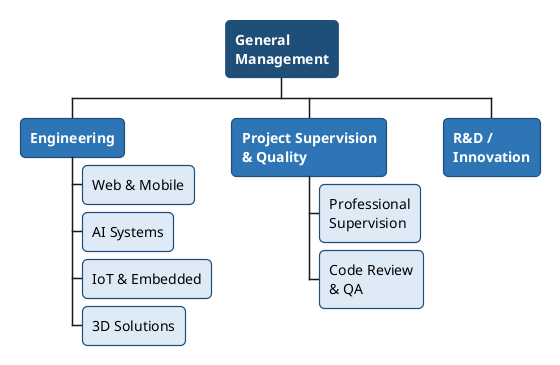
\includegraphics[width=0.85\linewidth]{img/org-neuralbey.png}
  \caption{Organisational chart of NeuralBey}
  \label{fig:org}
\end{figure}

\section{Project Presentation}

The project originated from an internal need identified at NeuralBey:
the Tunisian online-retail landscape lacks a modern, multi-vendor
platform that is both seller-friendly and equipped with the automation
features expected of contemporary marketplaces. Existing local
solutions are typically single-vendor stores or classified-ad sites,
and they offer limited tooling for moderation, content quality and
discovery.

A \emph{multi-vendor marketplace} is a platform on which independent
sellers operate their own stores within a shared environment governed
by a central operator. It differs from a \textbf{single-vendor store},
where the platform itself owns the inventory and the brand, and from a
\textbf{classified-ad site}, where the platform merely lists offers and
plays no part in transactions or quality control. A marketplace must
therefore reconcile three concerns simultaneously: \textbf{seller
autonomy} (each seller manages catalogue, branding and inventory),
\textbf{buyer trust} (the platform guarantees a baseline of product
authenticity and fulfilment) and \textbf{operator governance}
(administrators onboard sellers, moderate content, suspend stores and
curate featured selections).

Accordingly, three categories of target users were identified at the
scoping stage:

\begin{itemize}[leftmargin=*,itemsep=4pt]
  \item \textbf{Customer}, an end-user who browses the catalogue,
        places orders and tracks deliveries, expecting a fast,
        mobile-friendly experience with reliable search.
  \item \textbf{Seller}, a small or medium merchant who creates a
        store, manages a product catalogue and fulfils orders,
        expecting low onboarding friction and protection against
        unfair competition from low-quality listings.
  \item \textbf{Administrator}, the platform operator who reviews
        seller applications, moderates flagged content, curates
        featured stores, and intervenes when a store violates the
        marketplace rules.
\end{itemize}

\subsection{Study of Existing Solutions}

To position the proposed solution, three categories of competing
platforms were studied:

\begin{itemize}[leftmargin=*,itemsep=4pt]
  \item \textbf{Pan-African marketplaces (Jumia).} Jumia Tunisia is the
        most visible regional marketplace. It supports multiple vendors
        at scale and offers a polished customer experience, but seller
        onboarding is heavyweight and the platform is not tailored to
        small Tunisian merchants.
  \item \textbf{Classified-ad sites (Tayara, Affariyet).} Tayara
        dominates the local classified-ad market. It offers excellent
        discovery for sellers, but performs no escrow, no order
        management, no integrated payment and no quality moderation.
  \item \textbf{Single-vendor stores (MyTek, Wiki, etc.).} These are
        vertically integrated retailers that operate their own
        catalogue and cannot be used by independent sellers.
\end{itemize}

\subsection{Critique of Existing Solutions}

From the study above, four gaps emerged:

\begin{itemize}[leftmargin=*,itemsep=2pt]
  \item \textbf{No AI-assisted moderation.} On existing platforms,
        store and product verification are entirely manual, slow,
        inconsistent, and impractical at scale.
  \item \textbf{Heavyweight seller onboarding.} Pan-regional players
        require contractual paperwork unsuitable for small merchants.
  \item \textbf{Limited operator tooling.} Classified-ad sites have
        weak admin dashboards; single-vendor stores have none for
        external sellers.
  \item \textbf{Outdated technical foundations.} Several platforms still
        rely on monolithic stacks without modern CI/CD or
        infrastructure-as-code, making evolution costly.
\end{itemize}

Table~\ref{tab:competitors} summarises the comparison along the five
criteria that drove the design of the proposed solution. A check mark
(\ding{51}) indicates that the criterion is fully supported, a cross
(\ding{55}) that it is absent, and a tilde (\(\sim\)) partial support.

\begin{table}[H]
  \centering
  \caption{Comparative analysis of competing platforms}
  \label{tab:competitors}
  \begin{tabular}{lcccc}
    \toprule
    \textbf{Criterion}     & \textbf{Jumia} & \textbf{Tayara} & \textbf{Single-vendor} & \textbf{Proposed Solution} \\
    \midrule
    Multi-vendor model     & \ding{51} & \(\sim\)  & \ding{55} & \ding{51} \\
    AI verification        & \ding{55} & \ding{55} & \(\sim\)  & \ding{51} \\
    Admin dashboard        & \(\sim\)  & \ding{55} & \(\sim\)  & \ding{51} \\
    CI/CD pipeline (open)  & \ding{55} & \ding{55} & \(\sim\)  & \ding{51} \\
    Lightweight onboarding & \ding{55} & \ding{51} & \ding{55} & \ding{51} \\
    \bottomrule
  \end{tabular}
\end{table}

\subsection{Proposed Solution}

The proposed platform is a multi-vendor marketplace designed around
three pillars: a self-service seller experience, AI-assisted content
verification, and a modern, fully containerised deployment. It is built
as a single-page \textbf{React} application backed by a modular
\textbf{NestJS} API, with \textbf{MariaDB} as the relational store and
\textbf{n8n} acting as an orchestration layer for AI tasks.
Authentication is handled by \textbf{Better-Auth} with email
verification, and \textbf{Prisma} is used as the ORM. The full system is
packaged with Docker Compose, provisioned on DigitalOcean via Terraform,
and delivered through a GitHub Actions CI/CD pipeline.

Seven differentiators set the platform apart from the solutions
surveyed above:

\begin{itemize}[leftmargin=*,itemsep=2pt]
  \item \textbf{AI verification of stores and products} via an n8n
        workflow that calls a hosted large-language model and writes
        back a review flag together with a textual rationale.
  \item \textbf{Lightweight seller onboarding} through a seller
        application form reviewed by administrators, with a free tier
        offering a single store at zero cost.
  \item \textbf{Integrated administration tooling} (review, suspend,
        curate, cascade-delete) implemented as first-class features
        rather than database admin scripts.
  \item \textbf{Conversational data access} via a database-aware
        chatbot built on n8n, allowing administrators to query the
        platform in natural language.
  \item \textbf{AI-assisted storefront redesign}, sellers can
        regenerate their entire store visual identity from a
        natural-language prompt, powered by an n8n workflow and a hosted
        large-language model.
  \item \textbf{Store-wide and per-product sale promotions}: a seller can
        discount an entire store at once or put individual products on
        sale, with the percentage propagating automatically across
        product cards, store listings and search results and applying at
        checkout; when both apply, the larger discount always wins.
  \item \textbf{Modern DevOps foundations}, a pnpm monorepo, Docker
        Compose, Terraform on DigitalOcean and GitHub Actions CI/CD, 
        demonstrating production-grade engineering practices end to end.
\end{itemize}

The scope was agreed with the professional supervisor and bounded to
keep the deliverables clear:

\medskip
\noindent\textbf{In scope:} account creation and email verification;
the seller application workflow with admin review; store and product
CRUD with image upload; tag-based product recommendations with a
top-seller fallback; order placement, items and history; secure online
card payment at checkout; admin
moderation panels (store suspension, cascade-delete); AI verification
and chat assistant via n8n; store-wide and per-product percentage sales
with automatic badge propagation; AI-assisted storefront redesign; a premium tier
unlocking additional stores; and infrastructure-as-code deployment.

\medskip
\noindent\textbf{Out of scope} (deferred to future iterations):
a native mobile application; advanced fraud detection; on-premise LLM
hosting; multi-currency support; and a full-text search engine.

\section{Project-Management Methodology}

Every software project requires a methodological framework to organise
work, manage priorities and guarantee the delivery of a quality
product. This section justifies the choice of an agile method, 
\textbf{Scrum}, and presents its process, roles, events and
artefacts.

\subsection{Classical vs Agile Approaches}

Two major families of methods have historically competed: the
\textbf{classical} (predictive) approach and the \textbf{agile}
(adaptive) approach. The classical \emph{Waterfall} model divides the
project into strictly sequential phases, requirements, design,
development, testing, delivery, each fully validated before the next
begins. It suits projects whose requirements are stable and known in
advance, but it shows its limits as soon as the context evolves:
requirements are frozen at launch, the client sees a working product
only at the very end, and defects are detected too late to address
without significant impact.

Agility, born from the \textit{Agile
Manifesto}~(2001)~\cite{agilemanifesto}, champions collaboration,
adaptability and the continuous delivery of value. Rather than planning
the entire project upfront, work is organised into \textbf{short
iterations}, each producing a functional and tested increment.
Requirements are refined continuously from feedback, value is delivered
from the first iterations, and risks are identified and addressed early.

\subsection{Main Types of Agile Methodologies}

Several frameworks implement the agile principles, each with a different
emphasis, as summarised in Table~\ref{tab:agile}.

\begin{table}[H]
  \centering
  \caption{Main types of agile methodologies}
  \label{tab:agile}
  \begin{tabularx}{\textwidth}{|l|X|}
    \hline
    \rowcolor{tableHeader}
    \textcolor{white}{\textbf{Framework}} & \textcolor{white}{\textbf{Emphasis}} \\
    \hline
    Scrum & Organises work into time-boxed \emph{sprints} around three accountabilities and a small set of events; the most widely adopted agile framework. \\ \hline
    Kanban & Visualises the flow of work on a board and limits work-in-progress, favouring continuous flow over fixed iterations. \\ \hline
    Extreme Programming (XP) & Focuses on engineering practices such as pair programming, test-driven development and continuous integration. \\ \hline
  \end{tabularx}
\end{table}

\subsection{Why Scrum?}

Scrum~\cite{scrumguide} was selected because it offers the clearest
framework for delivering a substantial product in successive,
demonstrable increments while keeping requirements open to change. Its
sprint rhythm gives the project a regular cadence of planning and
review, its backlog provides a single prioritised source of truth for
the work, and its review events give the professional supervisor, 
acting as the stakeholder, frequent opportunities to steer the
product. These properties fit a project whose scope was expected to
evolve through the internship.

\subsection{The Scrum Process}

Scrum builds the product through a series of \textbf{sprints}: short,
fixed-length iterations at the end of which a potentially shippable
increment is delivered. Each sprint draws its work from the
\emph{Product Backlog} into a \emph{Sprint Backlog}, the work is built
and tested during the sprint, and the resulting increment is reviewed
with the stakeholder before the next sprint begins.
Figure~\ref{fig:scrum} illustrates this cycle.

\begin{figure}[H]
  \centering
  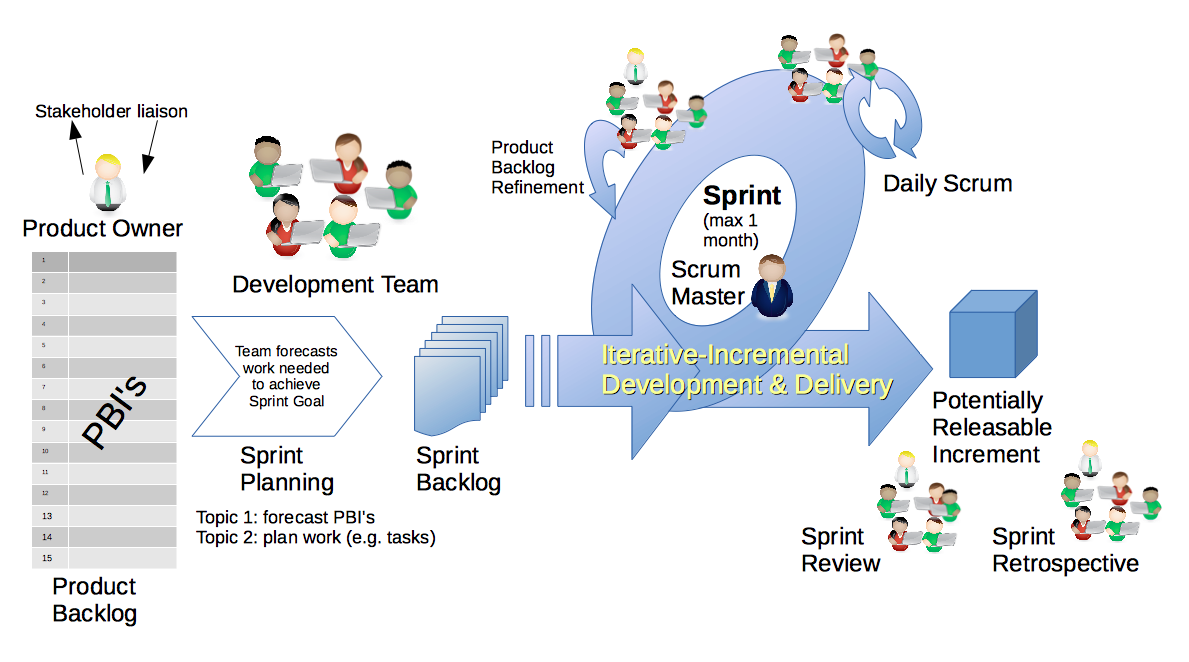
\includegraphics[width=0.9\linewidth]{img/scrum-framework.png}
  \caption{The Scrum framework: from the Product Backlog to a shippable increment}
  \label{fig:scrum}
\end{figure}

\subsubsection{Scrum Roles}

Scrum defines three accountabilities, which in this project were
distributed across two people as follows:

\begin{itemize}[leftmargin=*,itemsep=4pt]
  \item \textbf{Product Owner and Scrum Master}, owns the product
        vision, prioritises the backlog, ensures the framework is applied
        and removes impediments. These roles were held by the
        professional supervisor, \textbf{Mr.\ Mohammed Aziz Chibani}
        (NeuralBey), who also provided architectural guidance.
  \item \textbf{Development Team}, builds the increment. The entire
        technical realisation, analysis, design, implementation,
        testing and deployment, was carried out by the student,
        \textbf{Nadim Jebali}.
\end{itemize}

\subsubsection{Scrum Events}

The work was punctuated by Scrum's events:

\begin{itemize}[leftmargin=*,itemsep=2pt]
  \item \textbf{Sprint Planning}, selecting, at the start of each
        sprint, the backlog items to be delivered.
  \item \textbf{Daily Scrum}, a short daily checkpoint to track
        progress and surface impediments.
  \item \textbf{Sprint Review}, demonstrating the increment to the
        Product Owner and gathering feedback.
  \item \textbf{Sprint Retrospective}, reflecting on the process to
        improve the next sprint.
\end{itemize}

\subsubsection{Scrum Artefacts}

Three artefacts ensured transparency of the work:

\begin{itemize}[leftmargin=*,itemsep=2pt]
  \item \textbf{Product Backlog}, a prioritised list of all expected
        functionalities, maintained as user stories with MoSCoW
        priorities and complexity estimates (detailed in
        Chapter~\ref{chap:requirements}).
  \item \textbf{Sprint Backlog}, the subset of backlog items
        committed to the current sprint.
  \item \textbf{Increment}, a working, demonstrable version of the
        product delivered at the end of each sprint.
\end{itemize}

\section{Modelling Language}

To analyse and design the system, the project relies on the
\textbf{Unified Modeling Language} (UML)~\cite{umlspec}, the standard
graphical notation for specifying and visualising the artefacts of a
software system. UML offers complementary diagrams that capture both the
structural and the behavioural views of a system: \emph{use-case
diagrams} express the functional requirements from the actors'
perspective, \emph{class diagrams} describe the static domain model,
and \emph{sequence} and \emph{activity diagrams} depict dynamic
behaviour. The next chapter uses these diagrams to formalise the
requirements and the design of the platform.

\begin{figure}[H]
  \centering
  
\includegraphics[height=2.6cm,keepaspectratio]{img/uml-logo.png}
  \caption{The Unified Modeling Language (UML) logo}
  \label{fig:uml-logo}
\end{figure}

\section*{Conclusion}

This chapter established the foundations of the project. It introduced
NeuralBey, the host organisation, and the business motivation behind
building a modern Tunisian multi-vendor marketplace. A study of existing
platforms revealed four gaps, absent AI moderation, heavyweight
onboarding, weak admin tooling and outdated technical foundations, 
that the proposed solution directly addresses through its key
differentiators and bounded scope. Finally, the Scrum methodology and
the UML modelling language that frame the rest of the work were
presented. The following chapter formalises the requirements derived
from this context.
